\documentclass[a4paper,10pt]{article}
\usepackage{calc}
\usepackage[dvipsnames]{xcolor}
\usepackage{amsfonts}
\usepackage{latexsym}
\usepackage{placeins}
\ifx\pdftexversion\undefined
  \usepackage[dvips]{graphicx}
\else
  \usepackage[pdftex]{graphicx}
\fi
\usepackage{amssymb}
\usepackage{authblk}
\usepackage{amsmath}
\usepackage[cp1250]{inputenc}
%\usepackage[OT4]{fontenc}
\usepackage[T1]{fontenc}
\usepackage{graphicx,wrapfig,lipsum}
%\usepackage[a4paper]{geometry}
\pagestyle{empty}
%\usepackage{vmargin}
\usepackage{mathtools}


%\setpapersize{A4}
%\setmargins{3cm}       % margen izquierdo

%\addtolength{\textwidth}{3.9cm}


\usepackage{lineno}
%\linenumbers


\renewcommand{\textwidth}{15.5cm}
\addtolength{\oddsidemargin}{-1.7cm}
\renewcommand{\textheight}{24cm}
\addtolength{\topmargin}{-1.6cm}

\newcommand{\smalllineskip}{\baselineskip=15pt}
%\setlength{\parindent}{0.5cm}\setlength{\parskip}{2ex plus 0.3ex minus 0.1ex}
\setlength{\parindent}{0.5cm}\setlength{\parskip}{0ex plus 0.1ex minus 0.0ex}



\newcommand{\yt}{\ensuremath{y_{t}}}
\newcommand{\ttbar}{\ensuremath{t\bar{t}}}
\newcommand{\ttH}{\ensuremath{t\bar{t}H}}
\newcommand{\tH}{\ensuremath{tH}}
%\newcommand{\tHq}{\ensuremath{tHq}}
\newcommand{\tHq}{\tH}
\newcommand{\dileptau}{\ensuremath{2\ell+\tau_{had}}}


\begin{document}
	

%%%%%%%%%%%%%% PLEASE, DON'T MODIFY THIS PART	%%%%%%%%%%%%%%
\begin{center}
\vspace*{-2.2cm}
{\noindent\textsf{\textcolor{gray}{XXXVIII Reuni\'on Bienal de la RSEF  -- Murcia 2022}}}
\vspace{0.1cm}
\hrule
\vspace{0.1cm}		
\color{gray}{
\textsf{Two lines of space reserved to include}

\textsf{codes of the symposium and of this communication}
}
\end{center}
\vspace{0.6cm}
%%%%%%%%%%%%%% PLEASE, DON'T MODIFY THIS PART %%%%%%%%%%%%%%		
	

%%%%% SPACE TO INTRODUCE TITLE, AUTHORS AND FILIATION %%%%%
\begin{center}
\textbf{\LARGE\textsf{Search for associated production of a Higgs boson and 
a single-top quark in the \textit{2$\boldsymbol{\ell}$+$\boldsymbol{\tau_{had}}$} final state at 13$\,$TeV in ATLAS}}
\bigskip

{\large
\textsf{
S. Cabrera $^1$,
%F. Cardillo, $^1$, 
C. Escobar$^1$,
J. Guerrero$^1$,
%Mart\'inez-Agull\'o, Pablo$^1$,
%Mart\'inez-Agull\'o, P.$^1$,
{\textbf{P. Mart\'inez-Agull\'o}}$^{1,*}$
 %AuthorC$^3$
 }}
\medskip

%\textit{\textsf{{$^{\rm 1}$}DepartmentA, InstitutionAddressA, CountryA. {$^{\rm 2}$}DepartmentB, InstitutionAddressB, CountryB. {$^{\rm 3}$}DepartmentC, InstitutionAddressC, CountryC.}}

\textit{\textsf{{$^{\rm 1}$}Instituto de F\' isica Corpuscular (IFIC), 
 Centro Mixto Universidad de Valencia - CSIC, Valencia, Spain}}
\end{center}	
\vspace*{-0.2cm}

\centerline{\textsf{\small *e-mail: pablo.martinez.agullo@ific.uv.es}}
\bigskip
%%%%% END OF SPACE TO INTRODUCE TITLE, AUTHORS AND FILIATION %%%%%



%%%%% PLEASE WRITE YOUR ABSTRACT HERE %%%%%
The discovery of a Higgs boson by the ATLAS and CMS experiments in 2012 opened 
a new field for exploration in the realm of particle physics. In order to better understand 
the Standard Model (SM) of particle physics, it is of prominent interest to understand the Yukawa coupling of 
the Higgs boson to the top quark (\yt), being the latter the most massive fundamental particle 
and, consequently, the one with the largest coupling to the Higgs boson.

\begin{wrapfigure}{r}{5cm}
	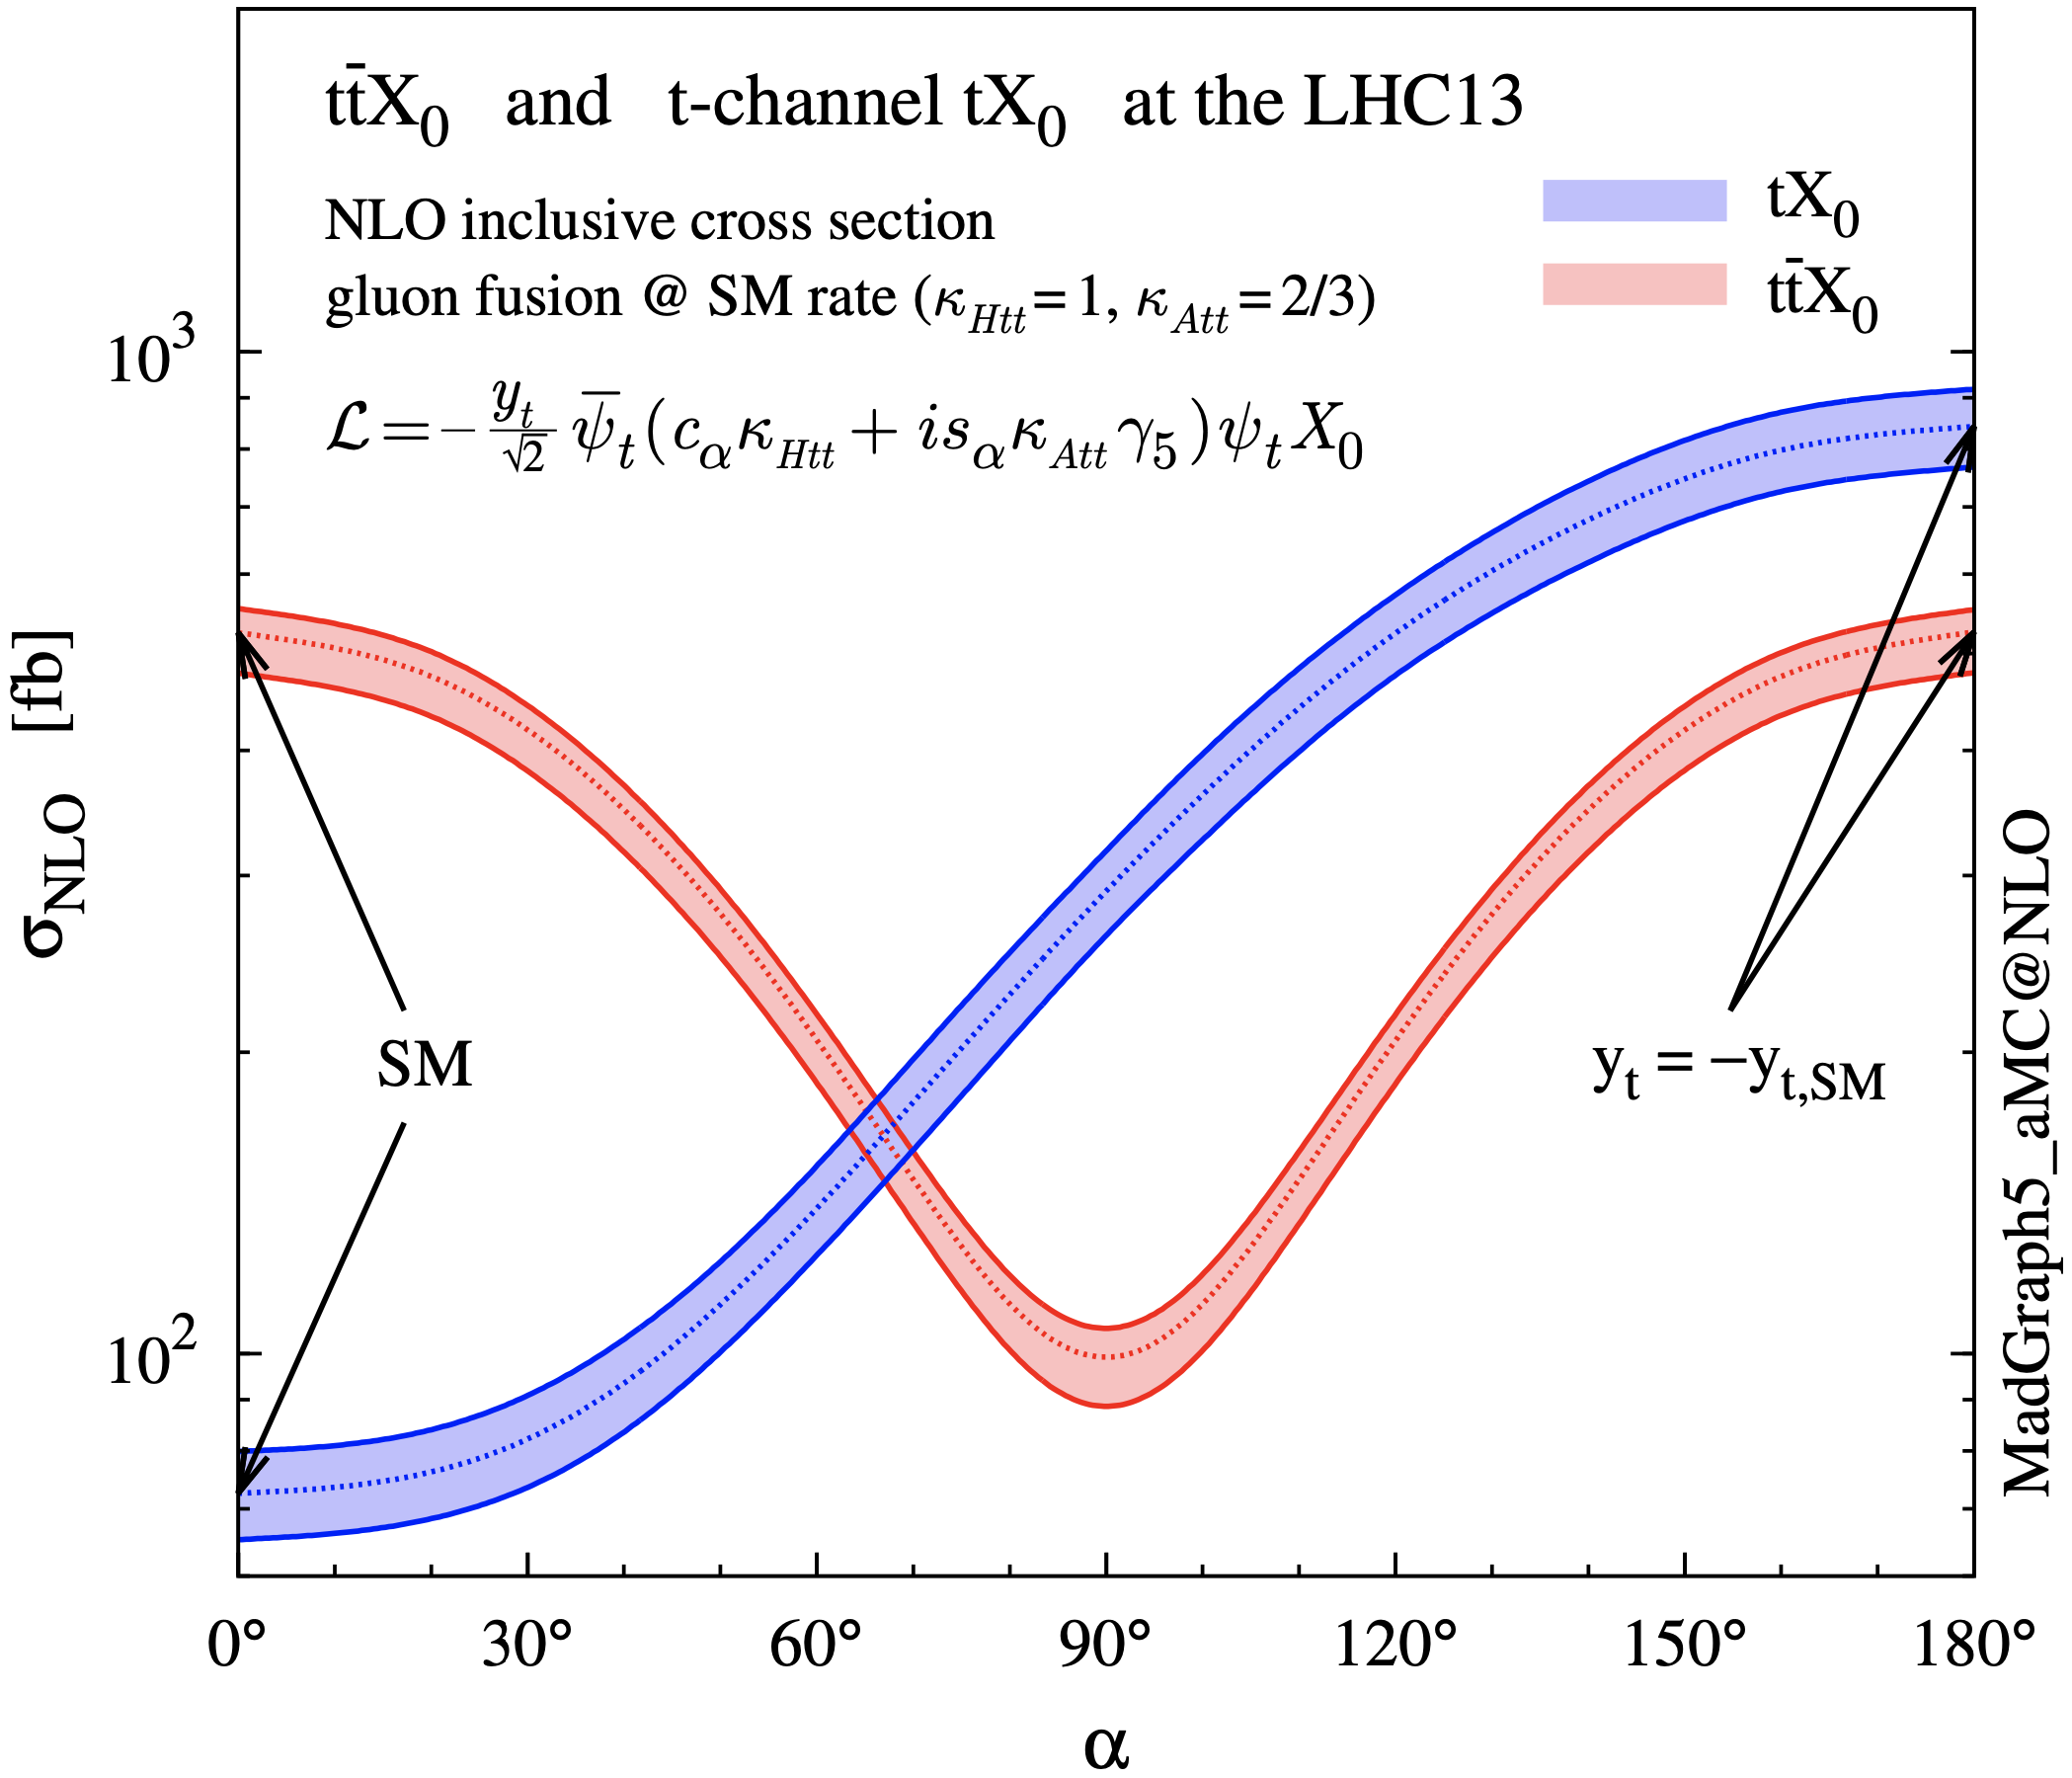
\includegraphics[width=5cm]{xsec_vs_yt_tH_ttH}
	%\caption{{\footnotesize A wrapped figure going nicely inside the text.}}
	{\footnotesize Figure 1. Production cross-section as a function of the CP mixing angle,
	$\alpha$, at NLO for $tX_{0}$ and $t\bar{t}X_{0}$, where $X_{0}$ represents a Higgs boson [1].}
	%\label{fig1:SeveralCurves}
\end{wrapfigure} 

The direct measurement of \yt$\,$ is only possible at the LHC via two associated
Higgs productions: with a top-quark-antiquark pair (\ttH) and with a single-top quark (\tHq). While the \ttH  
$\,$ just permits the determination of the magnitude of \yt, the only way of directly 
measuring its sign is through the \tHq$\,$ production (Fig.$\,$1). This is due to the fact that the two leading order 
Feynman diagrams for the \tHq$\,$production interfere with each other depending on the \yt$\,$ sign. 
Current experimental constrains on \yt$\,$ favour the SM predictions, but an opposite sign with 
respect to the expectations of the SM is not completely excluded yet [2].

In this work it is presented a search for the \tHq$\,$production in a final state with two light-flavoured-charged 
leptons (electrons or muons) and one hadronically-decaying tau lepton (named \dileptau$\,$ channel).
This analysis uses an integrated luminosity of 139 fb$^{-1}$ of proton-proton collision data at 
centre-of-mass energy of 13$\,$TeV collected by the ATLAS detector during LHC Run 2. 

This search is exceptionally challenging due to the extremely small cross-section of the \tHq$\,$process
(70$\,$fb), and of the \dileptau$\,$ final-state channel, in particular, which only accounts 
for a 3.5\% of the total \tHq$\,$production.
Therefore, the separation of the \tHq$\,$signal events from background events is done by means of 
machine-learning (ML) techniques using boosted-decision trees (BDT) to
define both signal (Fig.$\,$2) and control regions to constrain the most important background processes,
 which are those related
to top-quark-antiquark-pair production without and with and additional boson
(\ttbar, $t\bar{t}H$, $t\bar{t}W$ and $t\bar{t}Z$) and $Z$ boson plus jets.


\begin{wrapfigure}{l}{4.5 cm}
	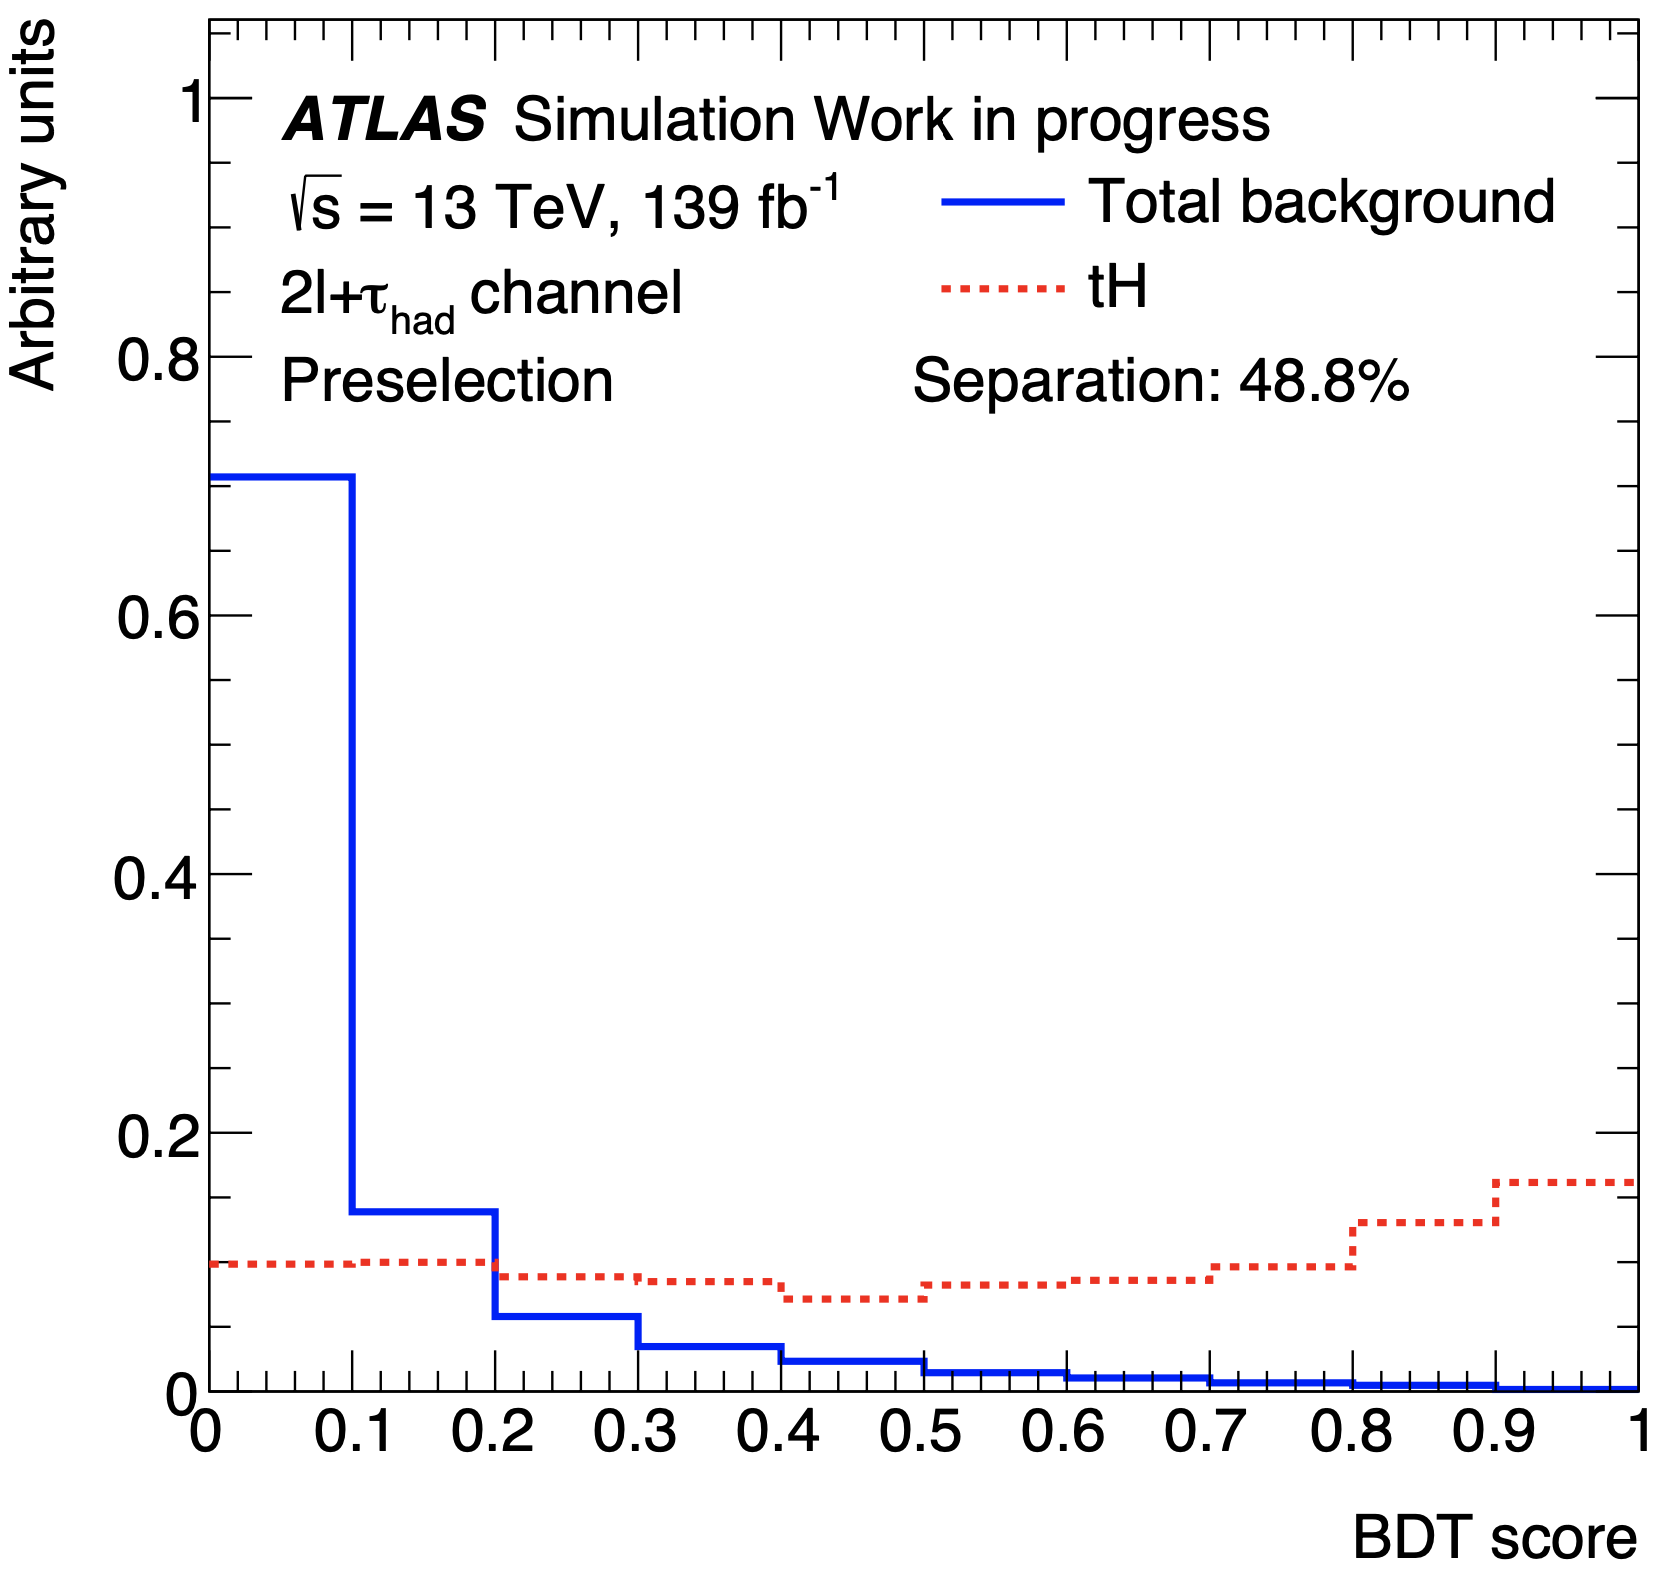
\includegraphics[width=4cm]{BDT_ScoreBDT_All_atLeast1b_croped}
	{\footnotesize Figure 2. Score of the BDT targeting \tHq$\,$ events over all backgrounds,
	used to define the signal region.}
\end{wrapfigure} 

Significant suppression of the background events with jets wrongly selected as leptons  
or non-prompt leptons originating from heavy-flavour decays
is achieved by demanding electrons and muons to pass strict identification and isolation requirements. 
Simultaneously, hadronic-$\tau$ leptons are demanded to pass the requirement of a
recurrent-neural-network-based discriminator to reduce misidentifications from jets.

The reconstruction of the events is also enhanced by similar ML methods
since in the scenario in which the light-flavour leptons have the same sign, a priori, 
it is not possible to determine which lepton is originated from the Higgs boson and 
which from the top quark.

The possible observation of an excess of signal events with respect to the SM prediction, would be an 
evidence of new physics in terms of CP-violating \yt$\,$ coupling.
\vspace{0.3 cm}

\medskip
{\small 
\noindent [1] F. Demartin, F. Maltoni, K. Mawatari and M. Zaro, \textit{Eur. Phys. J. C} \textbf{75}  (2015) 267. \newline
\noindent [2] CMS Collaboration, \textit{Eur. Phys. J. C} \textbf{81} (2021) 378
%\noindent [2] CMS Collaboration,  \textit{Phys. Rev. D} \textbf{99(9)},  (2019): 092005   \newline
}
%https://journals.aps.org/prd/pdf/10.1103/PhysRevD.99.092005
%Eur. Phys. J. C 75 (2015) 267
%Eur. Phys. J. C 81 (2021) 378

%Higgs production in association with a single top quark at the LHC, Eur. Phys. J. C 75 (2015) 267 (2015) (cit. on pp. 48–50)

%\medskip	
%{\footnotesize 
%\noindent \textbf{Acknowledgements}: \textcolor{red}{[delete if not applicable]}
%}


\end{document}

